\documentclass[a4paper,11pt]{article}

\usepackage[T1]{fontenc}

\usepackage[utf8]{inputenc}

\usepackage[italian]{babel}

\usepackage{graphicx}

\usepackage{indentfirst}

\usepackage{amsmath,amssymb}

\usepackage{enumitem} 

\newcommand{\virgolette}[1]{``#1''}

\usepackage[margin=1in]{geometry} %Smaller margins

\usepackage{lmodern} %Vector PDF

\usepackage{siunitx}

\usepackage{xcolor}

\usepackage{colortbl}

\usepackage{multirow}

\usepackage{rotating}

\usepackage{booktabs}

\usepackage{longtable}

\usepackage{graphicx}
\graphicspath{ {../../Immagini/} }

\usepackage{wrapfig}

\usepackage{siunitx} % Per unit� di misura in generale e la corretta rappresentazione dei numeri.

\usepackage{gensymb} % Per il simbolo di gradi

\begin{document}
	\section{Iter sperimentale}\label{proc}
	L'iter sperimentale può essere diviso nelle singole procedure utilizzate per compiere le diverse misure che erano l'obbiettivo dell'esperienza.
	
	\begin{wrapfigure}{r}{0.5\textwidth}
		\vspace{-2.2cm}
		\caption{Fotografia dell'apparato sperimentale}
		\vspace{0.2cm}
		\centering
		\label{apparato}
		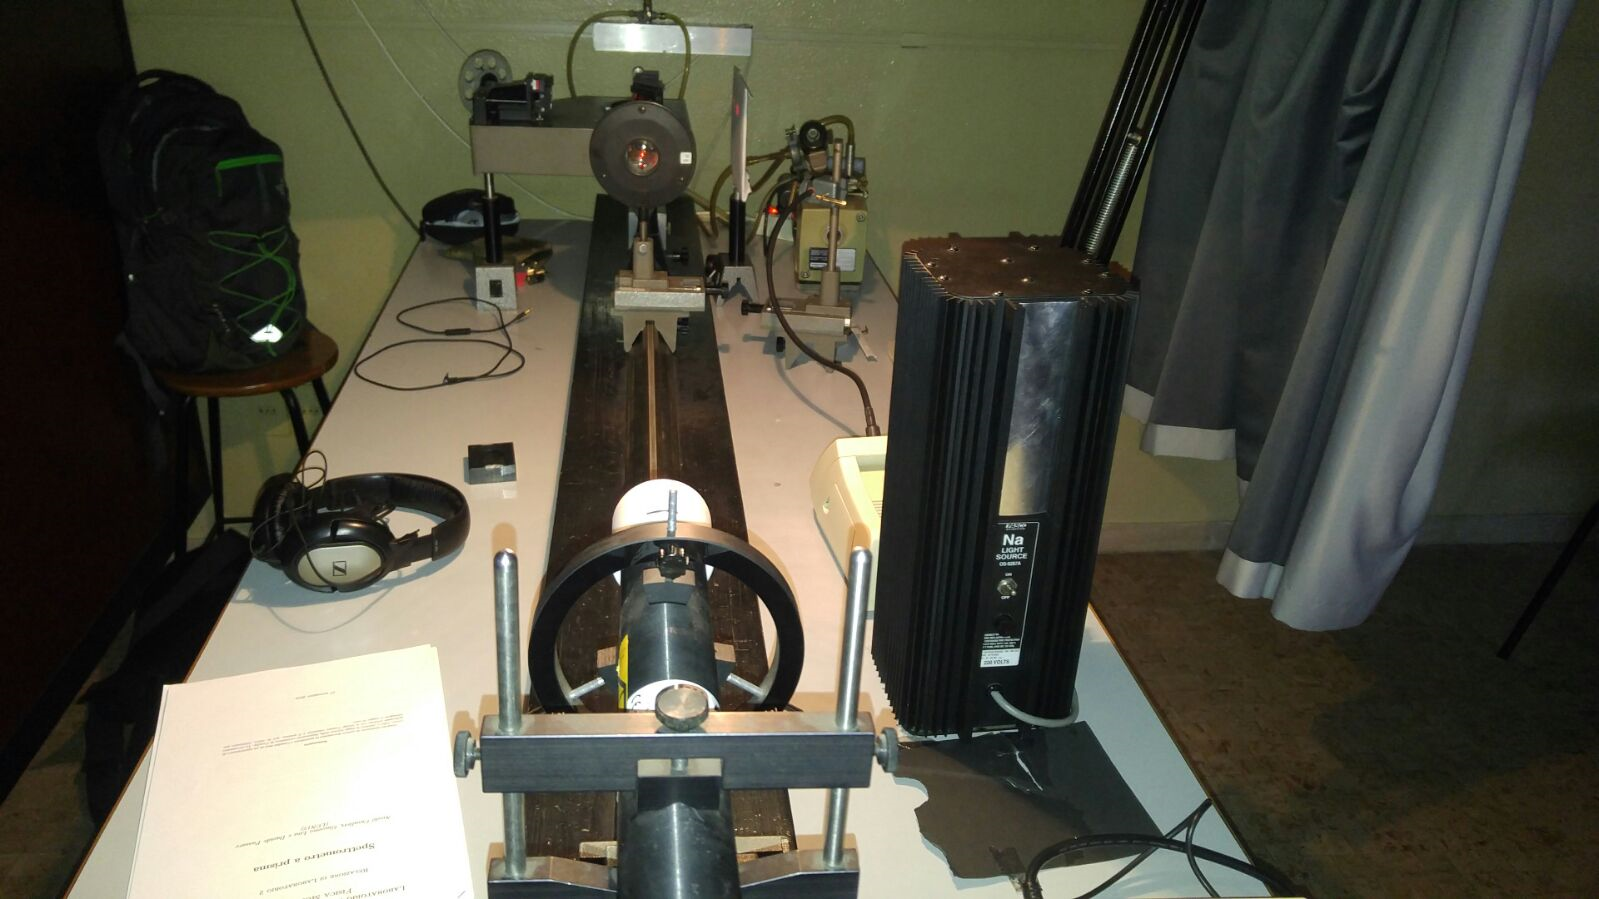
\includegraphics[width=0.48\textwidth]{apparato}
		\vspace{-1cm}
	\end{wrapfigure}
	
	\subsection{Lunghezza d'onda del laser}
	La prima parte dell'esperienza richiedeva una misura della lunghezza d'onda del laser. Questa operazione era sensata poiché il laser è un fascio di luce monocromatico e quindi dotato di una sola lunghezza d'onda.
	
	\subsubsection{Calibrazione dello specchio fisso}\label{calib}
	Per la misura della lunghezza d'onda del raggio laser è stata necessaria una calibrazione dell'interferometro volta al rendere lo specchio fisso perfettamente perpendicolare allo specchio mobile. Questo è stato fatto in due fasi. Per avere una condizione di perpendicolarità entro qualche primo è stata tolta la lente convergente. Sullo schermo si vedevano dei punti luminosi\footnote{Questi erano causati non interferenza ma da riflessioni \emph{parassite} dovute a riflessioni non volute degli innumerevoli specchi e lenti presenti nell'apparato.} ma i due corrispondenti alle riflessioni principali erano chiaramente distinguibili. Attraverso le viti dello specchio fisso si è quindi corretta la posizione dello specchio fino a quando i due punti luminosi non erano sovrapposti. Si è quindi proceduto inserendo tra la sorgente luminosa e il \emph{beam splitter}  la lente convergente. Sullo schermo erano quindi visibili i punti più luminosi sovrapposti e ingranditi. Attraverso un ulteriore aggiustamento dello specchio fisso si è potuti arrivare ad una condizione di quasi perfetta perpendicolarità, arrivando a vedere le frange di interferenza.
	
	\subsubsection{Misura}
	La misura della lunghezza d'onda ha sfruttato la possibilità di poter variare la posizione dello specchio mobile e quindi la differenza di cammino ottico dei raggi di luce. In questo modo era possibile controllare l'interferenza dei raggi luminosi e farli interferire in modo costruttivo o distruttivo. In particolare, affinché una frangia scura sullo schermo (corrispondente all'interferenza distruttiva) sostituisca una luminosa (interferenza costruttiva) è necessario spostare lo specchio di 
	\begin{equation}\label{delta}
		\Delta x = \dfrac{\lambda}{4n_a}
	\end{equation}
	dove $ \lambda $ è la lunghezza d'onda e $ n_a $ è l'indice di rifrazione dell'aria. Inoltre affinché una frangia chiara sostituisca una scura è necessario un ulteriore spostamento $ \Delta x $, da cui, per far si che una frangia chiara venga sostituita dalla successiva era necessario uno spostamento di $ 2\Delta x $.
	
	Poiché però la lunghezza d'onda era poco più grande della sensibilità dello strumento (la sensibilità era di $ \SI{0.2}{\micro\meter} $ mentre la lunghezza d'onda era dell'ordine di grandezza di $ \SI{100}{\nano\meter} $) per ottenere una misura con un errore accettabile era necessario far scorrere molte (circa $ \num{200} $) frange e dividere lo spostamento finale per il numero di frange viste. In questo modo rigirando la formula \ref{delta} si otteneva che:
	\begin{equation}\label{lambdana}
		\lambda=\dfrac{2n_a\Delta x}{N_1}		
	\end{equation}
	dove $ N_1 $ è il numero di frange contate e le altre osservabili sono come prima.
	
	\subsection{Indice di rifrazione dell'aria}
	Per la misura dell'indice di rifrazione dell'aria è stata usata la cameretta per il vuoto. Questa è stata posta in modo fisso tra la \emph{beam splitter} e lo specchio mobile ed è stata collegata ad una pompa per il vuoto. Il cambio dell'indice di rifrazione ha causato una differenza di cammino ottico. Una volta praticato il vuoto, attraverso una valvola a spillo si è lentamente fatto rientrare l'aria e contemporaneamente si è contato il numero di frange di luce che si alternavano. Al termine del rientro dell'aria il cammino ottico del fascio di luce passante per la cameretta del vuoto è variato della quantità:
	\begin{equation}\label{deltavuoto}
		\Delta s = 2(n_a-1)d
	\end{equation}
	dove $ d $ è la lunghezza della cameretta e $ n_a $ è l'indice di rifrazione dell'aria. Con un susseguirsi di $ N_2 $ fasci luminosi si ritrova quindi l'equazione \ref{indice_aria} che combinata con la \ref{lambdana} restituisce:
	\begin{equation}\label{lambda}
		\lambda=\dfrac{2d\Delta x}{N_1 d + N_2 \Delta x}
	\end{equation}
	\begin{equation}\label{na}
		n_a=\dfrac{N_1 d}{N_1 d + N_2 \Delta x}
	\end{equation}
	
	\subsection{Lunghezza dei pacchetti d'onda}
	Se la luce immessa nell'interferometro è non monocromatica, la luce emessa è costituita da pacchetti d'onda di lunghezza limitata non coerenti l'uno con l'altro. Posta quindi una sorgente di luce bianca, per misurare la lunghezza di uno di questi pacchetti era quindi necessario misurare lo spostamento tra una condizione di assenza di interferenza e l'altra. Questa misura si è rilevata essere la più difficoltosa in quanto le frange luminose erano difficilmente distinguibili e la condizione di interferenza era presente solo per un piccolissimo intervallo di differenza di cammino ottico.
	
	Una volta trovato però si è potuto misurare la differenza di cammino ottico che in questo caso equivaleva esattamente alla lunghezza del pacchetto di luce. 
	
	\subsection{Differenza di lunghezze d'onda}
	Come si era potuto verificare nell'esperienza dello spettrometro a reticolo il sodio presenta due frange luminose molto vicine l'una all'altra ma chiaramente distinte. Con l'interferometro di Michelson è stato possibile misurare con più precisione la differenza di lughezza d'onda dei due fasci. In particolare, poiché le lunghezze d'onda sono molto vicine l'una all'altra, per certi valori di differenza di cammino ottico si osserva che le frange luminose di una delle lunghezze d'onda si sovrappongono perfettamente a quelle dell'altra. L'immagine è quindi quella di una netta figura d'interferenza. Variando la differenza di cammino ottico, è possibie però raggiungere anche una posizione in cui le frange chiare di una lunghezza d'onda coprono quelle scure dell'altra, creando sullo schermo una luce diffusa. In questa condizione si è variata la differenza di cammino ottico di
	\begin{equation}\label{delta1}
		\Delta_1=2N_1\frac{\lambda_1}{2}=(2N_1+1)\frac{\lambda_2}{2}
	\end{equation}
	ovvero di un multiplo intero di una delle due lunghezze d'onda, e un numero dispari della metà della lunghezza d'onda dell'altro. Da questa relazione si ottiene quindi una equazione per ricavare $ N_1 $:
	\begin{equation}\label{N1}
		N_1=\dfrac{\lambda_1}{2\left(\lambda_2-\lambda_2\right)}\;.
	\end{equation}
	Con lo stesso ragionamento si può trovare che la figura di interferenza ritorna ad essere visibile dopo una differenza di cammino ottico di:
	\begin{equation}\label{delta2}
		\Delta_2=(2N_2+1)\frac{\lambda_1}{2}=2N_2\frac{\lambda_2}{2}
	\end{equation}
	e quindi 
	\begin{equation}\label{N2}
		N_2=\dfrac{\lambda_1}{\left(\lambda_2-\lambda_2\right)}=2N_1 \, .
	\end{equation}
	Sostituendo la \ref{N1} nella \ref{delta1} e la \ref{N2} nella \ref{delta2} si ottiene quindi che:
	\begin{equation}\label{deltas}
		\Delta_2=2\Delta_1=\dfrac{\lambda_2\lambda_1}{\lambda_2-\lambda_1}\approx\dfrac{\lambda^2}{\lambda_2-\lambda_1}
	\end{equation}
	dove $ \lambda $ è una stima di $ \lambda_1 $ o $ \lambda_2 $. Sperimentalmente però era molto più semplice distinguere le zone nella quale la diffusione era totale rispetto a quelle di interferenza. Quindi si è potuto facilmente misurare $ \Delta_2+\Delta_1=3\Delta_1 $ da cui si ottiene che:
	\begin{equation}\label{delta-lambda}
		\left(\lambda_2-\lambda_1\right)=\dfrac{3\lambda^2}{6\Delta_1}
	\end{equation}
\end{document}
